\section{Introduction}
\label{sec:intro}

Large language models (LLMs) need a lot of GPU memory. The 16-bit weights of a 7B-parameter model
take 15\,GB, and the key--value (KV) cache of every running request comes on top. To generate each
token, the GPU reads all the weights from memory, so generation is often limited by memory bandwidth
rather than by arithmetic~\cite{pope2023efficiently,gholami2024memorywall}. Quantization stores the
weights, and sometimes the activations, in 8 or 4 bits. Formats are named by their bit-width (W4A16
means 4-bit weights and 16-bit activations), which suggests a simple rule: fewer bits mean less
memory, faster generation and a small loss in quality.

This rule can fail in three places. \emph{Memory:} the embedding, the output layer, the KV cache and
the activations stay in 16 bits. \emph{Speed:} most formats must convert the weights back to 16 bits
(dequantize them) before each matrix multiply; this is free only if a fast kernel hides it while the
GPU waits for memory, and large batches make the GPU wait for arithmetic instead. \emph{Quality:}
the rounding error depends on the method and on the model.

Method papers report accuracy and kernel speed separately, usually on data-center
GPUs~\cite{frantar2023gptq,lin2024awq,frantar2025marlin,lin2025qserve}; comparison studies focus on
accuracy~\cite{jin2024comprehensive,li2024evaluating} or on one serving stack~\cite{kurtic2024give}.
But a user with one consumer GPU also picks a library, and the same format runs on very different
kernels in Hugging Face Transformers (bitsandbytes) and in vLLM (Marlin, CUTLASS).

We measure the whole trade-off on an NVIDIA RTX 5090, a 32\,GB consumer GPU, and answer the four
questions of our proposal. \textbf{Q1:} How much memory does quantization really save?
\textbf{Q2:} How do the time to first token (TTFT), the time per output token (TPOT) and the throughput
change? \textbf{Q3:} At which batch sizes and prompt lengths does a low-bit format become faster, or
slower, than BF16? \textbf{Q4:} How much quality does it cost? We test eight configurations on two
backends and five models (Qwen2.5 at 3B, 7B and 14B; Qwen3-8B and Qwen3-32B to check generality), and
explain the results with kernel benchmarks, a measured roofline and GPU profiles. Our main findings:

\begin{figure}[t]
\centering
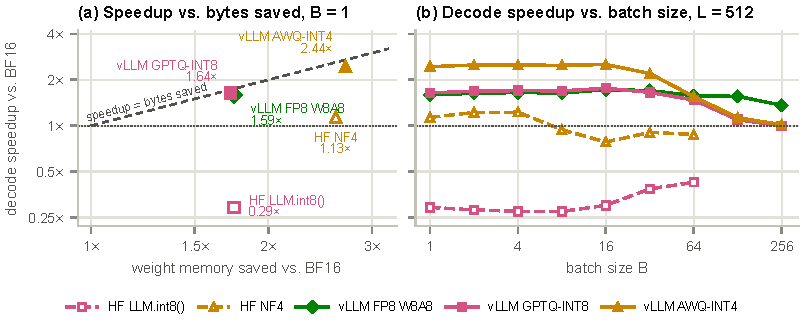
\includegraphics[width=\linewidth]{teaser_speedup}
\caption{\textbf{The bit-width does not predict the speedup.} (a)~Decode speedup over BF16 at batch
size~1 against the weight memory each format saves (Qwen2.5-7B, 512-token prompts). If decode time
were set only by the bytes read, every point would lie on the dashed line; the vLLM stack comes close,
the HF + bitsandbytes stack does not. (b)~As the batch grows, weight-only formats lose their gain; FP8 keeps it.}
\label{fig:teaser}
\end{figure}

\begin{itemize}
\item \textbf{Memory (Q1, \cref{sec:q1}).} 4-bit weights shrink Qwen2.5-7B by
  \WtNFSeven--\WtAWQSeven, not $4\times$, and the total saving drops to \MemBigNF{} with many tokens
  in flight. On vLLM the saved memory becomes KV cache (\KVratioAWQ{} more tokens).
\item \textbf{Speed (Q2, \cref{sec:q2}).} The implementation decides the speedup (\cref{fig:teaser}a): at
  batch size~1, vLLM's kernels turn \IdealAWQ--\IdealGQE\% of the byte saving into speed, NF4 only
  \IdealNF\%, and LLM.int8() is \INTeightslowdown{} slower than BF16.
\item \textbf{Crossover (Q3, \cref{sec:q3,sec:mechanism}).} Weight-only formats lose their speedup
  where decoding becomes compute-bound (\cref{fig:teaser}b; AWQ-INT4 at $B\approx\AWQcross$), while
  FP8 wins at every batch size. On HF, kernel launches on the CPU limit small models.
\item \textbf{Quality (Q4, \cref{sec:q4,sec:general}).} 8-bit formats stay within \EightKernMax{}
  points of BF16; 4-bit formats cost \MFourAbsMin--\MFourAbsMax{} MMLU points, more on smaller
  models, yet at a fixed memory budget a larger 4-bit model wins.
\end{itemize}

We release the harness, the raw data and the scripts that produce every number, table and figure in
this report.\footnote{\url{https://github.com/zz9tf/6359-SYS-ARCHITECT-course-work}}
